\documentclass{beamer}
\usepackage[utf8x]{inputenc}
\usepackage{graphicx}
\usepackage{tikz}
\graphicspath{{./../../img/}}

\usepackage[T1]{fontenc}

\usetheme{TUM}

\title[Research Graph]{Research Graph}

\author[Guerin, Silva, Zimmerer]{Fiona Guerin, Alvaro Silva, Andreas Zimmerer}
\institute{Technical University of Munich}

\date{10 March 2020}

% Customize alert
\setbeamercolor{alerted text}{fg=TUMZusatzfarbeBlau3}
\setbeamerfont{alerted text}{series=\bfseries}

\begin{document}
\maketitle

\begin{frame}{Vision}
    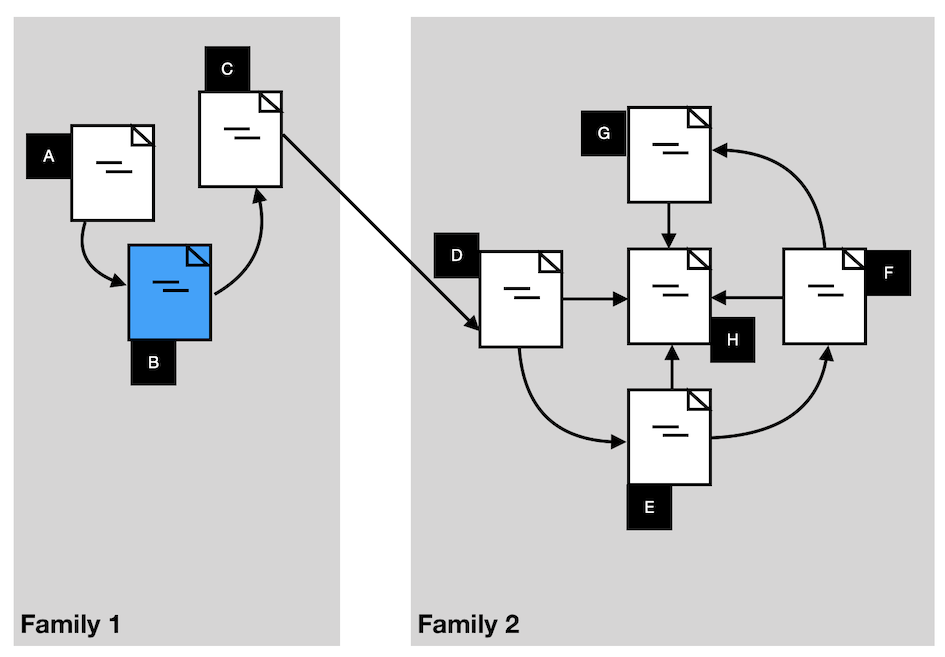
\includegraphics{img_02.png}
\end{frame}

\begin{frame}{Research Graph: Planned Features}
    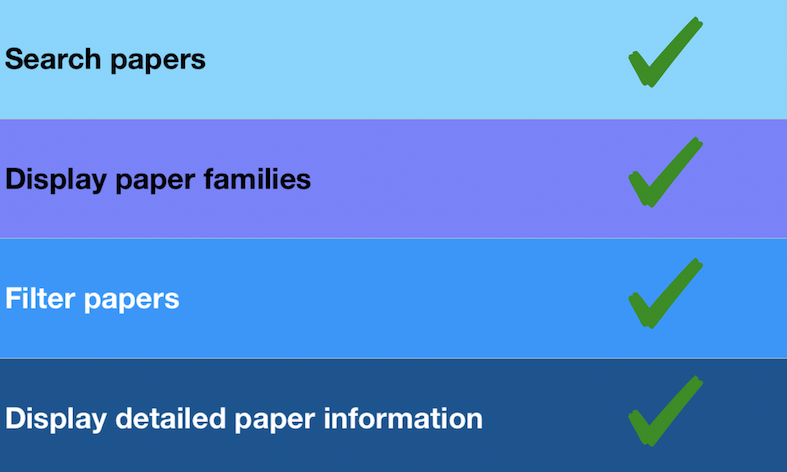
\includegraphics{img_19.png}
\end{frame}

\begin{frame}{Research Graph: Extra Features}
    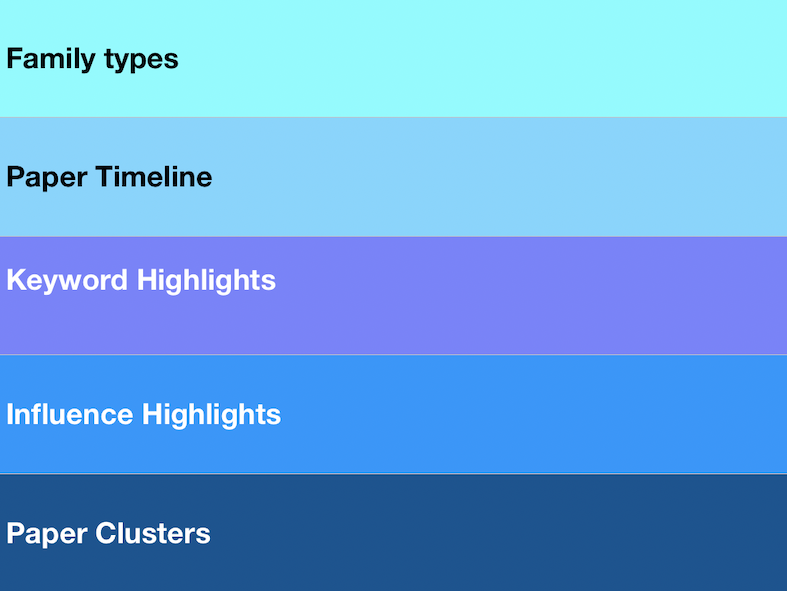
\includegraphics{img_20.png}
\end{frame}

\begin{frame}{Mockup}
    \url{Link: https://github.com/Jibbow/research-paper-graph/blob/master/doc/img/mockup.gif}
\end{frame}

\begin{frame}{Demo}
    \url{Link: https://research-paper-graph-frontend.herokuapp.com/}
\end{frame}

\begin{frame}{Performance}
    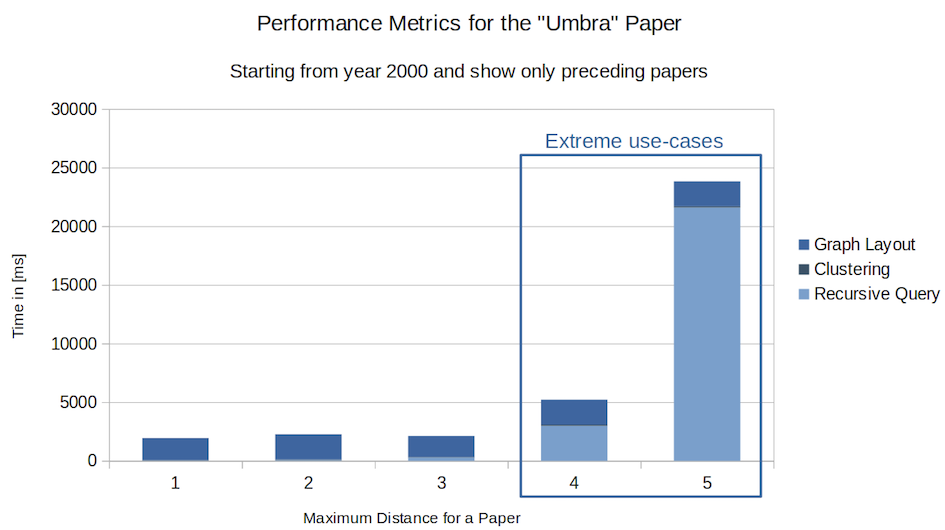
\includegraphics{img_25.png}
\end{frame}

\begin{frame}{Responsibilities: Andreas}
    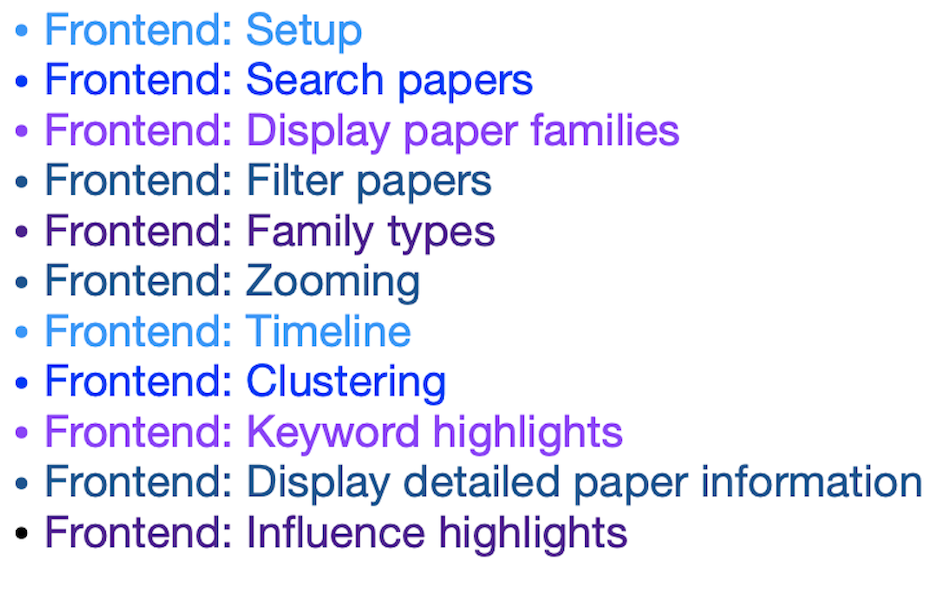
\includegraphics{img_22.png}
\end{frame}

\begin{frame}{Responsibilities: Alvaro}
    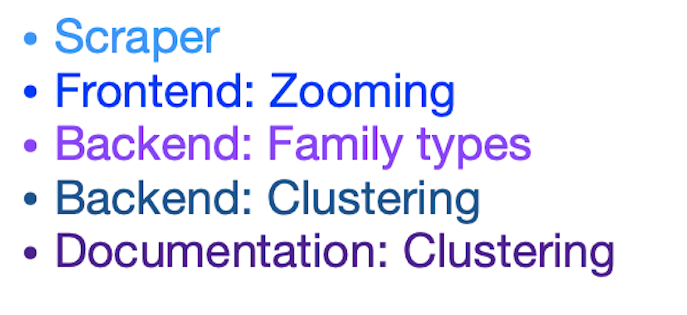
\includegraphics{img_23.png}
\end{frame}

\begin{frame}{Responsibilities: Fiona}
    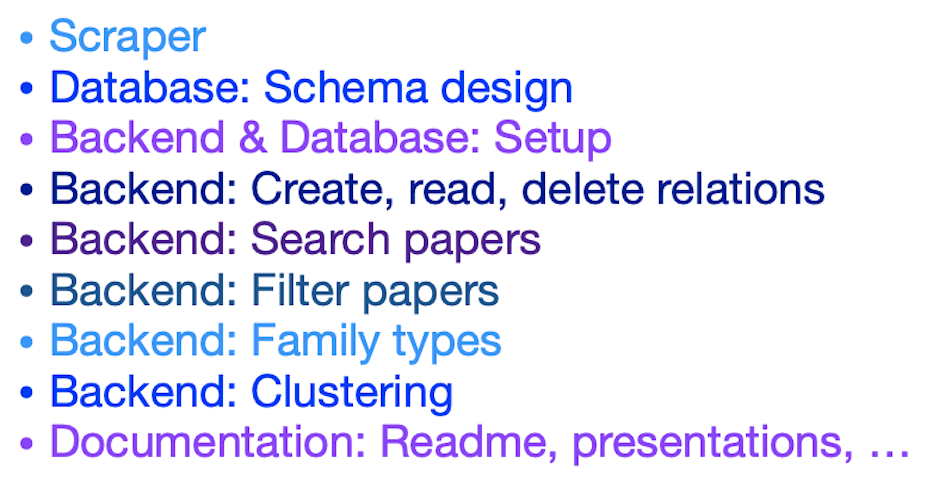
\includegraphics{img_24.png}
\end{frame}

\begin{frame}{Lessons Learned}
    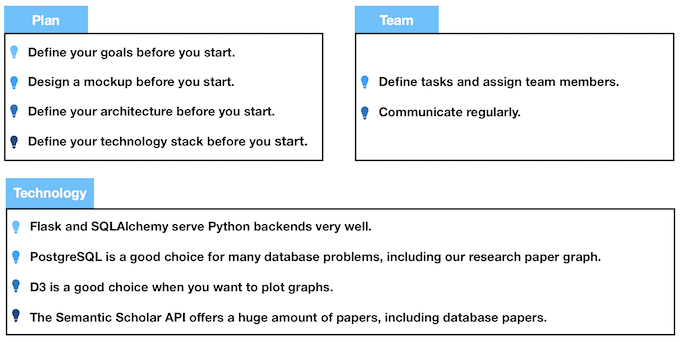
\includegraphics{img_21.png}
\end{frame}

\begin{frame}{Github}
    \url{https://github.com/Jibbow/research-paper-graph}
\end{frame}

\begin{frame}{Thank you}
    
\includegraphics{img_05.png}
\end{frame}

\end{document}
